\section{Introduction}

The vision of model driven development (MDD)
\cite{schmidt:modelDrivenEngineering,stahl:mdsd}
even predates the definition of the Unified Modelling Language (UML); yet it
has historically been implemented with little success. With a cleaner separation of
architecture from design as envisaged by the Object Management Group's (OMG),
Model Driven Architecture (MDA) \cite{siegel:developingInMDA,frankel:enterpriseMDA}
together with semantically richer modelling languages like UML 2.x and stronger
tools support for MDD, the interest in MDD has increased considerably.

Yet there are a number of open issues which hold back the widespread adoption of MDD.
The first issue is the lack of a clear definition on what needs to be included in the
Platform Independent Model (PIM). Braek and Melby \cite{braek:modelDrivenServiceEngineering}
define a minimal requirements without specifying precisely the required components
for the PIM. This paper attempts to specify more concretely the artifacts which should
be included in a PIM.

The second issue is the lack of standards available to define the implementation architecture
and technologies required for the implementation mapping. This aspect is then often addressed in
a tool specific way like, for example, the cartridges approach of Andro-MDA. Usually this aspect
is further simplified by MDA tools supporting a specific set of reference architectures like
Java-EE, CORBA, CCM, JBI/SOA or Microsoft.Net.

The third issue slowing down the wide-spread adoption of MDA is the virtual lack of
a well defined, practical analysis and design methodology together with a
precise definition of the inputs and outputs
including the artifacts which must be included in the specification of a PIM.
which must be produced to define a required with specified inputs and outputs.

In this paper we will try and formulate some steps towards addressing the first
two issues. We will formulate some requirements for the PIM and will present
the Use-Case, Responsibility Driven Analysis and Design (URDAD)
\cite{solms:urdad}, a simple, algorithmic analysis and design methodology
which can be used by domain experts such as business analysts to generate the
PIM. The domain experts need not have an understanding of the implementation
architecture and technologies.

%--------------------------------------------------------------------

\subsection{Analysis and design methodologies}

Historically, URDAD has grown out of Responsibility Driven Design (RDD)
methodology pioneered by Rebecca Wirfs-Brock and Brian Wilkerson (see
\cite{wirfs-brock:responsibilityDrivenApproach},  and
\cite{wirfs-brock:objectDesign} \cite{wirfs-brock:designSimplicity}) and has
been influenced by the approaches of step-wise refinement \cite{wirth:stepWiseRefinement}
and top-down design \cite{martin:agileSoftwareDevelopment}.

But, while all of these are design approaches, URDAD provides an algorithmic
analysis and design methodology with the following characteristics:
\begin{enumerate}
  \item Both, requirements and design are step-wise refined.
  \item URDAD specifies the steps of the design methodology with
			well-defined inputs and outputs for each step, making the process repeatable
			and predictable.
  \item Generation of services contracts for the service providers required at any
			level of granularity enforcing a technology-neutral approach as well as
			pluggability and testability at any level of	granularity.
	\item Work flow logic at any level of granularity is factored out of the service
			providers for that level of granularity, enforcing decoupling of role players
			across levels of granularity.
	\item URDAD provides an explicit approach to fixing the levels of granularity.
   \item URDAD explicitly aims to generate a technology and architecture neutral design
			representing MDA's PIM.
\end{enumerate}

One of the benefits of having a standard design methodology generating a set of
predictable artifacts for the PIM, is that it simplifies the mapping from the platform
independent model (PIM) to the platform specific model (PSM), i.e.\ the methodology defines
standard set of source elements for the model transformations.

%------------------------------------------------------------------------------

\subsection{MDA-based development methodologies}

URDAD is usually embedded within an iterative realization or development process. Reviews of some
MDA-based development methodologies can be found in \cite{bercovici:businessArchitectureToSoa}
A typical model driven development process is shown in figure \ref{fig:developmentProcess}. 
Note that the technology neutral business process design is performed by business analysis. 
The technical team comprising both, architecture and implementation (development), 
is responsible for the realization of the business process within the chosen architecture and technologies.

\begin{figure}
  \centering
  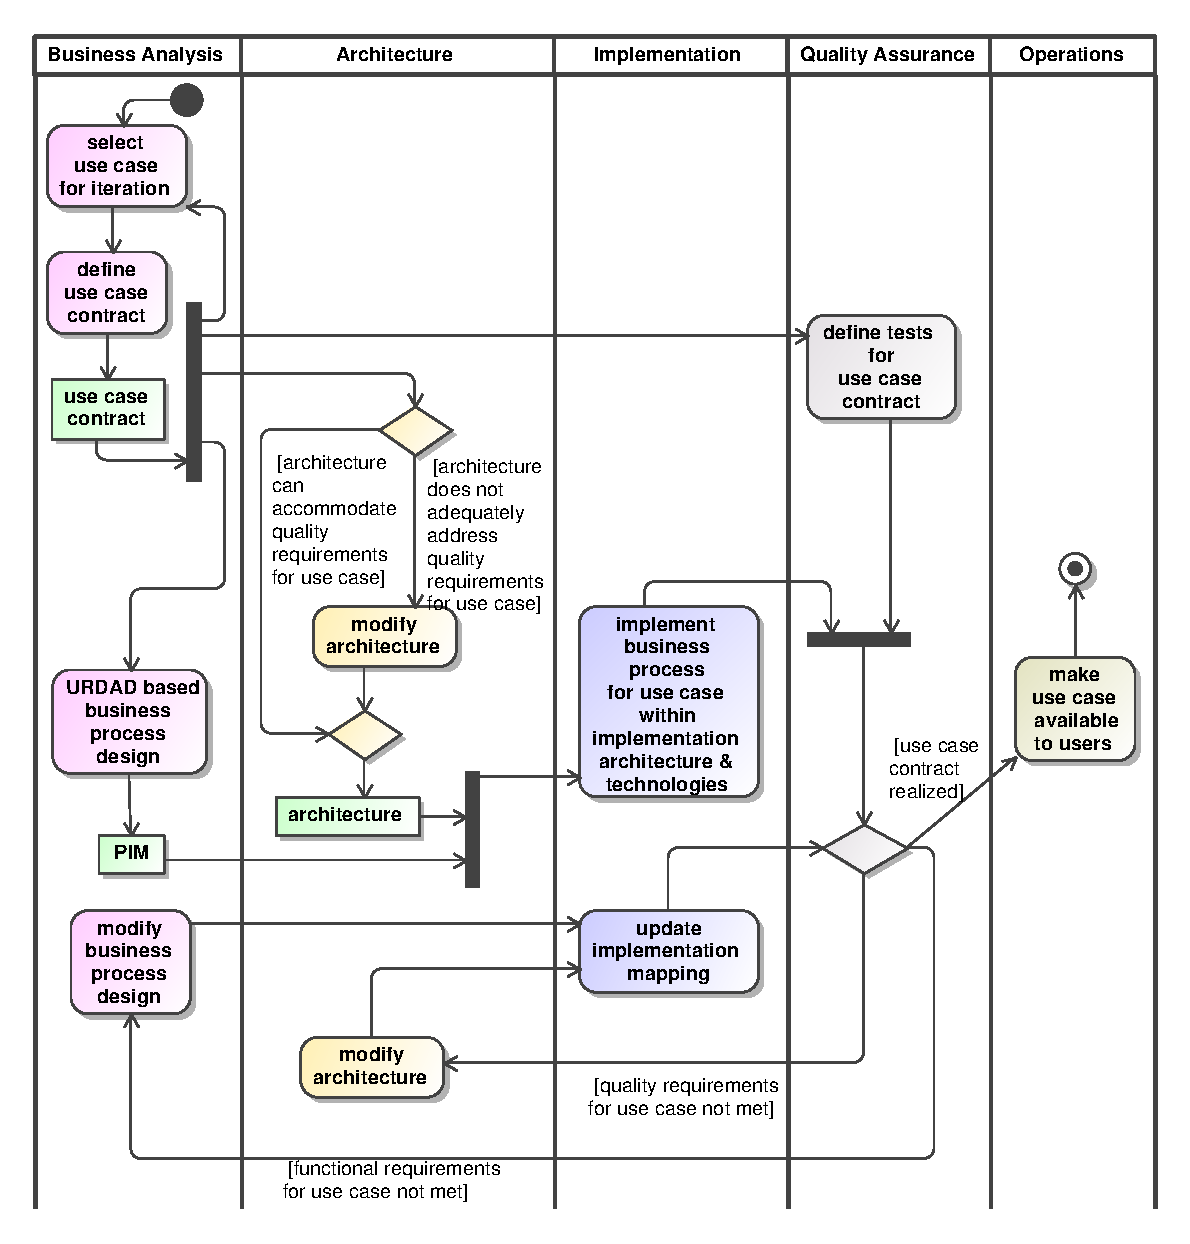
\epsfig{file=developmentProcess.eps, scale=0.6}
  \caption{Outline of a model driven development process.}
  \label{fig:developmentProcess}
\end{figure}

After passing quality assurance and actual deployment, operations takes over the management of the
business process execution.

%-------------------------------------------------------------------------------

\subsection{Real-life experiences with URDAD}

URDAD has been developed and taught to both business analysts and software designers since 2002.
More than a dozen of companies have been and are using URDAD for their technology neutral analysis
and design methodology. Some of these have decided to enforce the URDAD methodology as an organization
wide standard. Examples of such companies include
\begin{itemize}
  \item {\em Strate} (http://www.strate.co.za), the authorized Central Securities Depository (CSD) for the electronic settlement of all financial instruments in South Africa.
	\item {\em AllCare Administrators} (http://www.allcare.co.za), a medical aid administrator, and
	\item {\em Multichoice} (http://www.multichoice.co.za), the premier digital media provider in South Africa.
\end{itemize}
Strate's experiences with URDAD have been partially documented in \cite{klopper:compareSoftwareMethodologies}.

The main reasons for standardizing on URDAD typically include
\begin{itemize}
  \item higher productivity achieved through the algorithmic process and the separation of technical concerns,
  \item standardized outputs of the analysis and design process with improved quality and consistency, and
  \item the benefits of having business processes documented in a technology neutral way.
\end{itemize}

Core difficulties often experienced include
\begin{itemize}
  \item a resistance to adopting UML for business process documentation, and
  \item challanges around separating the business processes from the currently employed technologies, and
  \item insufficient understanding of the methodology leading to inconsistent and low-quality results.
\end{itemize}
